\documentclass[11pt]{article}
\usepackage[english]{babel}
\usepackage[utf8]{inputenc}
\usepackage{johd}
\usepackage{ragged2e}
\usepackage{array}
\setlength{\parindent}{0em} 


\begin{document}


\thispagestyle{empty}


\begin{figure}[!h]
\centering

\includegraphics{images/uzh_logo.pdf}\\\
\end{figure}
\vspace{1cm}

\begin{center}
\huge {Cryptocurrencies and the risk-free rate}
\end{center}
\vspace{1cm}

\begin{center}
\large \textbf{Final Project}\\
\vspace{0.5cm}
Digital Tools for Finance (L) (03SMDFOEC008)\\
Department of Banking and Finance, University of Zurich\\
Igor Pozdeev
\end{center}
\vspace{1cm}

\begin{center}
\large \textbf{Authors}\\
\vspace{0.5cm}
Jakob Pirs (XX-XXX-XX, jakob.pirs@uzh.ch)\\

Nina Erminia Cantoni (17-709-221, ninaerminia.cantoni@uzh.ch)\\

Rohit Koonireddy (XX-XXX-XX, rohit.koonireddy@bf.uzh.ch)\\

Yunxiang Guo (XX-XXX-XX, yunxiang.guo@uzh.ch)\\
\end{center}
\vspace{1cm}

\begin{center}
\large \textbf{Abstract}\\
\vspace{0.5cm}
\begin{justify}
This paper investigates the tie between the risk free rate (approximated by the 10 year treasury yield) and the returns of the cryptocurrencies Bitcoin, Etherium, XRP and Litecoin, as well as the cryptocurrency market (approximated by CMC Crypto 200 Index by Solactive). For this purpose a data set is created using the yahoo API. The paper finds weak covariance and neglegible correlation. It is to conclude, that the cryptocurrency returns are not related to spikes in the risk free rate.
\end{justify}
\end{center}
\vspace{1cm}


\begin{center}
\vfill{}
\par\end{center}

\begin{center}
\renewcommand{\today}{\ifcase \month \or January\or February\or March\or   April\or May \or June\or July\or August\or September\or October\or November\or  December\fi, \number \year} 

\begin{center}
\large{\today}
\end{center}
\end{center}

\pagebreak{}
\pagebreak{}


\tableofcontents
\pagenumbering{roman}
\setcounter{page}{2}
\pagebreak{}


\listoftables
\pagebreak{}


\pagenumbering{arabic}
\setcounter{page}{1}


\section{Context and motivation}

The goal of this paper is to analyze the correlation between the 10 year treasury yield and cryptocurrencies. The 10 year treasury rate is the yield one receives for investing in US government securities with a maturity of 10 years. It is a common proxy for the risk free rate. The risk free rate is a basic component of most pricing theories and thus a very relevant factor in the finance world. This paper will shed light on the influence of the risk free rate on the price of cryptocurrencies by analyzing price data over a period of 5 years. It will also be examined, wether the cryptocurrency market as a whole is influenced.
\\

To answer the research question, this paper looks at four different cryptocurrencies, namely Bitcoin, Etherium,  XRP (by Ripple) and Litecoin. Find an overview of the four currencies in Table \ref{tab1} below.


\begin{table}[H]
\textbf{\caption{\label{tab1} Cryptocurrencies overview}}
\centering % Label your table accordingly
\begin{tabular}{>{\centering\arraybackslash}m{0.15\textwidth} >{\centering\arraybackslash}m{0.15\textwidth} >{\centering\arraybackslash}m{0.15\textwidth} >{\centering\arraybackslash}m{0.15\textwidth} >{\centering\arraybackslash}m{0.15\textwidth}}
\hline
Logo & Name & Symbol & Market Cap as of Nov 25, 2022 & Ranking as of Nov 25, 2022\\
\hline
\\

\includegraphics[width=0.1\textwidth]{images/Bitcoin.png} &  Bitcoin & BTC & \$ 318 bn & 1\\
\\

\includegraphics[width=0.05\textwidth]{images/ETH.png} & Ethereum & ETH & \$ 149 bn & 2\\
\\

\includegraphics[width=0.1\textwidth]{images/XRP.png} & XRP & XRP & \$ 20 bn & 7\\
\\

\includegraphics[width=0.1\textwidth]{images/LTC.png} & Litecoin & LTC & \$ 6 bn & 13\\
\\
\hline
\end{tabular} 
\newline

\note{\textit{Note.} Data as of November 25, 2022, retrieved from CoinGecko (www.coingecko.com).}
\end{table}
\newline


Besides these single cryptocurrencies, we also consider a cryptocurrency index. By looking at an index, we can replicate the cryptocurrency market as a whole and abstract from indiosyncratic risks of single currencies. The index that was considered is the CMC Crypto 200 Index by Solactive. The CMC Crypto 200 Index tracks the price movementes of the top 200 cryptocurrencies by market capitalization. It was launched at year end 2018 and is calculated and distributed by Solactive AG. The index is published in USD. The calculation of the index price is conducted on a daily basis \citep{CMC200}. As of November 2022, the four cryptocurrencies analyzed in this paper (Bitcoin, Etherium,  XRP and Litecoinwere) were within the 13 cryptocurrencies with the highest market capitalization and therefore also part of the CMC Crypto 200 (see Table \ref{tab1}).




\section{Data set}
\subsection{Data set}
\\

TEST IS THIS STILL HERE
\\

This paper is based on a data set consisting of prices of the four cryptocurrencies of interest Bitcoin, Etherium, XRP and Litecoin, of the CMC Crypto 200 Index and of the 10 year US treasury bond. The data was sourced form Yahoo! through its Application Programming Interface (API). For each of the above mentioned assets, the daily (adjusted) closing price was retrieved. The data set spans from January 1, 2018 to November 12, 2022. As the CMC Crypto 200 Index was launched only at year end 2018, there is a lack of data with respect to the index for the first year within our sample. These missing data points led to NaN values in our data set. Therefore, a first step consisted of cleaning the data set and replacing NaN values with zeros.

The final data set as well used for the calculations of the dependency measures is openly accessible on our GitHub, allowing for reproduction of our exact results:
\paragraph{Object name} data\_adjusted\_small.parquet
\paragraph{Format names and versions} Parquet
\paragraph{Creation date} 2022-11-15
\paragraph{Dataset creators} Jakob Pirs (co-author)
\paragraph{Language} English
\paragraph{API} yahoo 
\paragraph{Repository name} GitHub 
\paragraph{Repository path} https://github.com/ncanto/group-work.git


%Here you can provide, if applicable, information about the dataset(s) whose creation, collection, management, access, processing or analysis have been discussed in this paper, following this schema:
%\paragraph{Object name} Typically the name of the file or file set in the repository.
%\paragraph{Format names and versions} E.g., ASCII, CSV, Autocad, EPS, JPEG, Excel, SQL, etc.
%\paragraph{Creation dates} The start and end dates of when the data was created (YYYY-MM-DD).
%\paragraph{Dataset creators} Please list anyone who helped to create the dataset (who may or may not be an author of the data paper), including their roles (using and affiliations).
%\paragraph{Language} Languages used in the dataset (i.e., for variable names etc.).
%\paragraph{License} The open license under which the data has been deposited (e.g., CC0). 
%\paragraph{Repository name} The name of the repository to which the data is uploaded. E.g., Figshare, Dataverse, etc. 
%\paragraph{Publication date} If already known, the date in which the dataset was published in the repository (YYYY-MM-DD).


\subsection{Characteristics of the variables}
To get a feel for the data we looked at the means of all variables (Figure \ref{fig:mean}) and the standard deviations (Figure \ref{fig:std}) of the cryptocurrencies. ETH has clearly the highest closing price on average, the 10 year treasury bond (referred to as TNX) the lowest. Regarding standard deviation, XRP has the highest value.


\begin{figure}
\centering
\begin{minipage}{.5\textwidth}
  \centering
  \caption{Means}
  \label{fig:mean}
  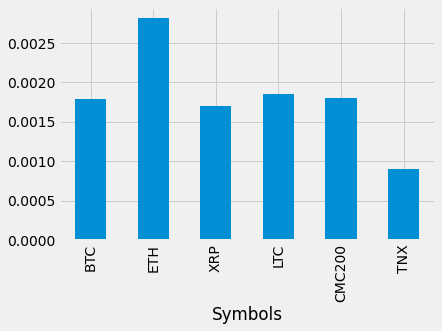
\includegraphics[height=5.8cm,keepaspectratio]{images/mean.png}
  \note{\textit{Note.} Own representation.}
\end{minipage}%
\begin{minipage}{.5\textwidth}
  \centering
  \caption{Standard deviations}
  \label{fig:std}
  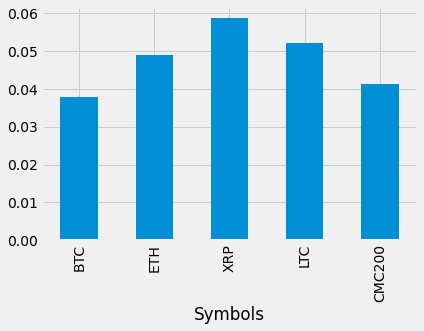
\includegraphics[height=5.8cm,keepaspectratio]{images/std.png}
  \note{\textit{Note.} Own representation.}
\end{minipage}
\end{figure}

Lastly, in Figure \ref{fig:mov_treasury} we tracked the price movement of the 10 year treasury yield and in Figure \ref{fig:mov_crypto} the price movement of the cryptocurrencies.

\begin{figure}
    \centering
    \caption{Covariance}
    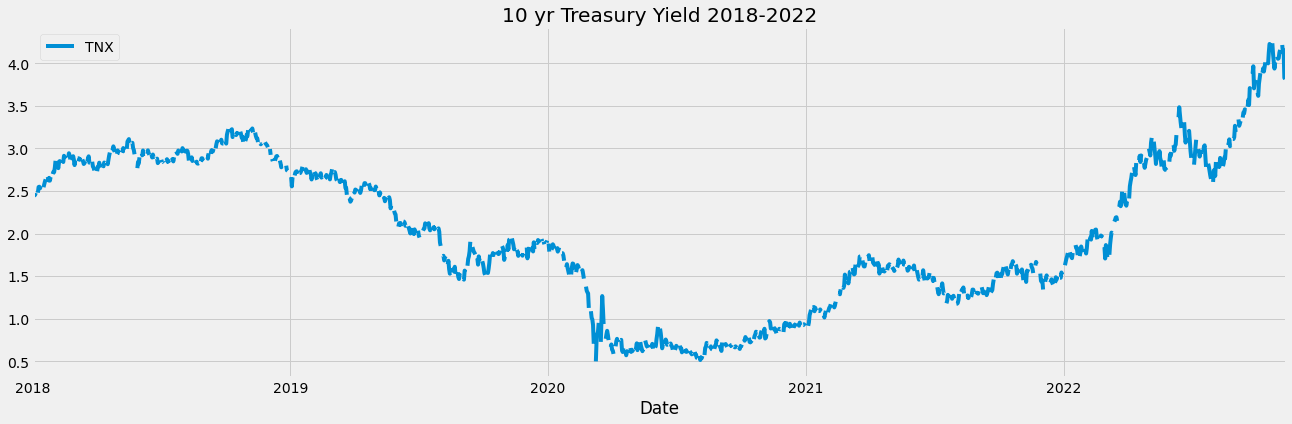
\includegraphics[width=\textwidth,height=\textheight,keepaspectratio]{images/movement_treasury.png}
    \label{fig:mov_treasury}
    \note{\textit{Note.} Own representation.}
\end{figure}

\begin{figure}
    \centering
    \caption{Covariance}
    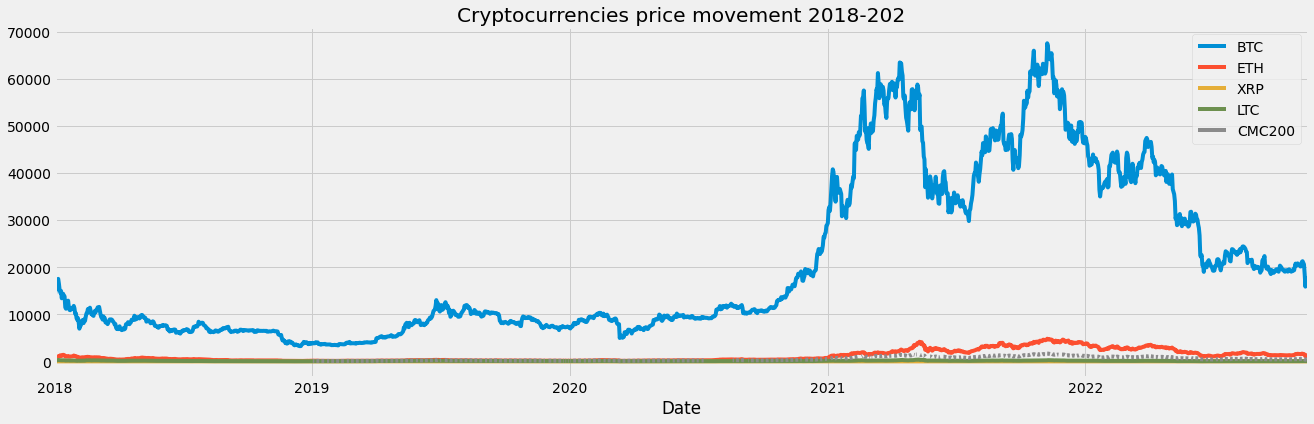
\includegraphics[width=\textwidth,height=\textheight,keepaspectratio]{images/movement_crypto.png}
    \label{fig:mov_crypto}
    \note{\textit{Note.} Own representation.}
\end{figure}


\section{Method}
The goal of this paper is to assess whether there is any connection between the 10 year treasury yield and the return of cryptocurrencies. To detect a potential connection we relied on two classical statistical measures: covariance and correlation.

\subsection{Covariance}
The covariance is a measure to relate the movement of two random variables. A positive covariance indicates that the two variables move in the same direction. A negative covariance means that the variables move inversely, meaning that if one increases, the other one will decrease and vice versa. Therefore, covariance measures the direction of a relation. The covariance is given by the following formula \citep{cov}:
\begin{center}
   \large $cov_{x,y}=\frac{\sum_{i=1}^{N}(x_{i}-\bar{x})(y_{i}-\bar{y})}{N-1}$
\end{center}
By calculating the Covariance we can examine the direction of a potential relationship between the 10 year treasury yield and the cryptocurrencies.

\subsection{Pearson's Correlation}
Similarly to the covariance, also the correlation is a measure for relationship. The correlation measures the strength of a relationship. The correlation coefficient lives on the interval between negative one and one. The higher the absolute value, the stronger is the observed relationship. A correlation of zero indicates no relationship between the observed variables. Therefore, this measure is very interesting for our research question. Depending on the correlation we can assess how strong the relationship between the 10 year treasury yield and the cryptocurrencies is (if any).\\

First, we assess the Pearson's correlation. The Pearson coefficient will will measure any linear relationships between the variables. There is a linear relationship when a change in the first variable causes a proportional change in the second variable. \citep{corr}


\subsection{Spearman's Correlation}
As we have seen above, the Pearson's correlation has its limits. Namely it is limited at measuring linear relationships. We therefore also introduce a second correlation measure, called the Spearman's correlation. The Spearman’s correlation coefficient extends the concept to non-linear, monotonic functions. Simply put, monotonic functions are functions that do not change direction but can have different steepness throughout. \citep{corr}


\subsection{Implementation}
The analysis was conducted using the programming language Python, making use of its functionalities. For the computations we relied on the \emph{pandas} package. We calculated the covariances within our data set using the \emph{data.cov()} function. Similarly, correlation was computed using the \emph{data.corr()} function, with specifications \emph{method='pearson'} and \emph{method='spearman'} accordingly. These are basic functions available in many programming languages. To ensure robustness of results, it is advisable to have a look at the documentation of the functions when using a different programming language, to ensure the functions are equal to the ones used in this paper.



\section{Results and discussion}
#The correlation between the 10yr treasury yield and other cryptocurrencies is very weak and shows negligible correlation.
#The interesting fact is if we compare BTC to other cryptos we see very high positive correlation.


#As seen from the results the correlation between the 10yr treasury yield and other cryptocurrencies is very weak
#For them to be at least moderatily correlated, the Spearman correlation coefficient would have to be greater than 0.40 in absolute terms.
#We conclude that there is no significant correlation between interest rate hikes and cryptocurrency exchange rates


\section{Implications/Applications}
Provide information about the implications of this research and/or how it can be applied.


\newpage


\bibliographystyle{johd}
\bibliography{bib}

\end{document}